% Shared standalone design for the editable figure reconstructions.
\documentclass[tikz,border=5pt,10pt]{standalone}
\usepackage[T1]{fontenc}
\usepackage[utf8]{inputenc}
\usepackage{newpxtext,newpxmath}
\usepackage[scaled=.94]{sourcesanspro}
\usepackage{pgfplots}
\pgfplotsset{compat=1.18}
\usetikzlibrary{arrows.meta,calc,positioning,decorations.pathreplacing,
  decorations.markings,patterns,matrix,shapes.geometric,fit,backgrounds,
  intersections,angles,quotes}
\definecolor{ink}{HTML}{203746}
\definecolor{accent}{HTML}{146C78}
\definecolor{muted}{HTML}{667780}
\definecolor{signalred}{HTML}{B94B44}
\color{ink}
\tikzset{>=Latex,line width=.8pt,
  every node/.style={font=\small},
  axis/.style={->,draw=muted,line width=.5pt},
  guide/.style={draw=muted,dashed,line width=.45pt},
  curve/.style={draw=accent,line width=1pt},
  marker/.style={circle,fill=accent,inner sep=1.5pt},
  labelbox/.style={fill=white,inner sep=2pt}}

\begin{document}
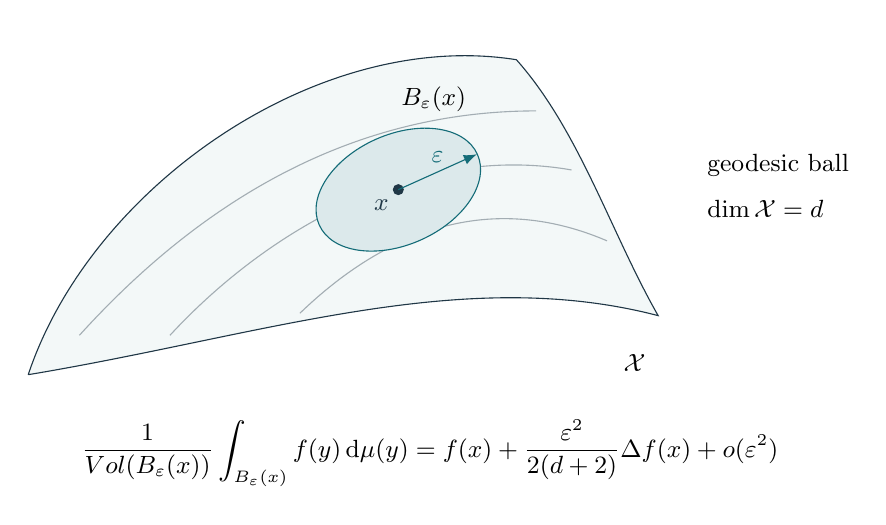
\begin{tikzpicture}[x=1cm,y=1cm]
\path[draw=ink,fill=accent!5] (0,0)..controls(.8,2.4)and(3.7,4.4)..(6.2,4.0)..controls(7.0,3.1)and(7.4,1.8)..(8.0,.75)..controls(5.5,1.4)and(3.0,.5)..(0,0);
\draw[muted!60] (.65,.5)..controls(2.1,2.1)and(4,3.35)..(6.45,3.35);
\draw[muted!60] (1.8,.5)..controls(3,1.8)and(4.9,2.95)..(6.9,2.6);
\draw[muted!60] (3.45,.78)..controls(4.25,1.55)and(5.6,2.45)..(7.35,1.7);
\path[draw=accent,fill=accent!15,rotate around={24:(4.7,2.35)}] (4.7,2.35) ellipse(1.1 and .7);
\fill[ink] (4.7,2.35) circle(2pt) node[below left] {$x$};
\draw[->,accent] (4.7,2.35)--(5.7,2.8) node[midway,above] {$\varepsilon$};
\node at (5.15,3.5) {$B_\varepsilon(x)$};\node at (7.7,.15) {$\mathcal X$};
\node[anchor=west,align=left] at (8.5,2.4) {geodesic ball\\[2mm]$\dim\mathcal X=d$};
\node at (5.1,-1.0) {$\displaystyle\frac{1}{\operatorname{Vol}(B_\varepsilon(x))}\int_{B_\varepsilon(x)}f(y)\,\mathrm{d}\mu(y)=f(x)+\frac{\varepsilon^2}{2(d+2)}\Delta f(x)+o(\varepsilon^2)$};
\end{tikzpicture}
\end{document}
